\documentclass[10pt,a4paper]{article}
\usepackage[margin=1.75cm,headheight=21pt]{geometry}
\usepackage[T1]{fontenc}
\usepackage[utf8]{inputenc}
\usepackage{lmodern}
\usepackage{microtype}
\usepackage{amsmath,amssymb}
\usepackage{booktabs,longtable,tabularx,array,multirow}
\usepackage{enumitem}
\usepackage{multicol}
\usepackage{graphicx}
\usepackage{tikz}
\usetikzlibrary{arrows.meta,positioning,fit,shapes.geometric,calc}
\usepackage[most]{tcolorbox}
\usepackage{listings}
\usepackage{xcolor}
\usepackage{fancyhdr}
\usepackage{titlesec}
\usepackage{hyperref}
\usepackage{bookmark}
\usepackage{lastpage}

% RootCastle-inspired brand system
\definecolor{RCNavy}{HTML}{071521}
\definecolor{RCBlue}{HTML}{087EA4}
\definecolor{RCCyan}{HTML}{25C2D7}
\definecolor{RCOrange}{HTML}{F59E0B}
\definecolor{RCInk}{HTML}{17212B}
\definecolor{RCGray}{HTML}{5B6873}
\definecolor{RCLight}{HTML}{EEF4F7}
\definecolor{RCGreen}{HTML}{15803D}
\definecolor{RCRed}{HTML}{B42318}

\hypersetup{
  colorlinks=true,
  linkcolor=RCBlue,
  urlcolor=RCBlue,
  citecolor=RCBlue,
  pdftitle={REI SignalLab 2.1 --- Product Wiki},
  pdfauthor={RootCastle},
  pdfsubject={Digital signal processing and spectral instrumentation documentation}
}

\pagestyle{fancy}
\fancyhf{}
\lhead{\textcolor{RCNavy}{\textbf{ROOTCASTLE}}\enspace\textcolor{RCBlue}{/ REI SignalLab 2.1}}
\rhead{\textcolor{RCGray}{Product Wiki}}
\lfoot{\textcolor{RCGray}{Engineering Beyond Boundaries}}
\rfoot{\textcolor{RCGray}{\thepage\ / \pageref{LastPage}}}
\renewcommand{\headrulewidth}{0.6pt}
\renewcommand{\headrule}{\hbox to\headwidth{\color{RCCyan}\leaders\hrule height \headrulewidth\hfill}}
\renewcommand{\footrulewidth}{0pt}

\titleformat{\section}{\Large\bfseries\color{RCNavy}}{\thesection}{0.65em}{}[\vspace{2pt}\color{RCCyan}\titlerule]
\titleformat{\subsection}{\large\bfseries\color{RCBlue}}{\thesubsection}{0.6em}{}
\titleformat{\subsubsection}{\normalsize\bfseries\color{RCInk}}{\thesubsubsection}{0.55em}{}
\titlespacing*{\section}{0pt}{1.35em}{0.65em}
\titlespacing*{\subsection}{0pt}{1.05em}{0.4em}
\setlength{\parindent}{0pt}
\setlength{\parskip}{0.55em}
\setlist{nosep,leftmargin=1.5em,topsep=0.3em}
\setcounter{tocdepth}{2}

\newcolumntype{Y}{>{\raggedright\arraybackslash}X}
\newcolumntype{L}[1]{>{\raggedright\arraybackslash}p{#1}}
\renewcommand{\arraystretch}{1.18}

\newtcolorbox{rcbox}[1][]{enhanced,breakable,colback=RCLight,colframe=RCBlue,
  boxrule=0.6pt,arc=1.5mm,left=2.5mm,right=2.5mm,top=2mm,bottom=2mm,#1}
\newtcolorbox{warningbox}[1][]{enhanced,breakable,colback=RCOrange!8,colframe=RCOrange,
  boxrule=0.8pt,arc=1.5mm,title={Operational note},fonttitle=\bfseries,coltitle=RCNavy,#1}
\newtcolorbox{trustbox}[2][]{enhanced,breakable,colback=#2!7,colframe=#2,
  boxrule=0.8pt,arc=1.5mm,#1}

\lstdefinestyle{rcstyle}{
  basicstyle=\ttfamily\small,
  backgroundcolor=\color{RCNavy},
  basicstyle=\ttfamily\small\color{white},
  keywordstyle=\color{RCCyan}\bfseries,
  stringstyle=\color{RCOrange},
  commentstyle=\color{white!60},
  showstringspaces=false,
  breaklines=true,
  frame=single,
  rulecolor=\color{RCBlue},
  numbers=left,
  numberstyle=\tiny\color{white!45},
  xleftmargin=1.5em,
  framexleftmargin=1em,
  columns=fullflexible
}
\lstset{style=rcstyle}

\newcommand{\product}{REI SignalLab 2.1}
\newcommand{\code}[1]{\nolinkurl{#1}}
\newcommand{\status}[2]{\textcolor{#1}{\textbf{[#2]}}}

\begin{document}
\pagenumbering{roman}

% Cover
\begin{titlepage}
\pagecolor{RCNavy}
\color{white}
\begin{tikzpicture}[remember picture,overlay]
  \fill[RCCyan] (current page.north west) rectangle ([yshift=-5mm]current page.north east);
  \fill[RCBlue] ([xshift=-22mm]current page.south east) rectangle (current page.north east);
  \draw[RCCyan!35,line width=0.4pt] ([xshift=12mm,yshift=25mm]current page.south west)
    sin ++(25mm,6mm) cos ++(25mm,-6mm) sin ++(25mm,-6mm) cos ++(25mm,6mm)
    sin ++(25mm,6mm) cos ++(25mm,-6mm) sin ++(25mm,-6mm) cos ++(25mm,6mm);
  \foreach \x in {0,...,10}{
    \draw[RCBlue!28,line width=0.3pt] ([xshift=12mm+12*\x mm,yshift=17mm]current page.south west) -- ++(0,28mm);
  }
\end{tikzpicture}

\vspace*{12mm}
{\fontsize{16}{18}\selectfont\bfseries ROOTCASTLE}\par
{\color{RCCyan}\large Engineering Beyond Boundaries}\par

\vfill
{\color{RCCyan}\large DIGITAL SIGNAL PROCESSING \textbullet\ SPECTRAL INSTRUMENTATION}\par
\vspace{5mm}
{\fontsize{35}{39}\selectfont\bfseries REI SignalLab 2.1}\par
\vspace{3mm}
{\fontsize{22}{26}\selectfont Product Wiki}\par
\vspace{8mm}
{\large Typed DSP graphs, numerical verification, and industrial vibration analysis}\par

\vfill
\begin{tabular}{@{}ll@{}}
\textcolor{white!60}{Document} & Detailed English product and engineering guide\\
\textcolor{white!60}{Edition} & 2.1 / August 2026\\
\textcolor{white!60}{Maintainer} & RootCastle\\
\textcolor{white!60}{Website} & \href{https://rootcastle.com}{rootcastle.com}
\end{tabular}
\vspace*{18mm}
\end{titlepage}
\nopagecolor
\pagenumbering{arabic}

\begin{rcbox}[title={Document scope},fonttitle=\bfseries]
This wiki describes the public \product{} application and repository as reviewed on 5 August 2026. It covers end-user operation, DSP behavior, data trust labels, graph projects, scripting facilities, APIs, deployment, maintenance, and known boundaries. The public implementation is the source of truth; deployments may differ by configuration or commit.
\end{rcbox}

\tableofcontents
\newpage

\section{Product overview}

\product{} is a browser-based laboratory suite for signal synthesis, transformation, filtering, spectral analysis, visualization, reproducible signal-flow experiments, and industrial machinery vibration analysis. It combines a React interface with a FastAPI/SciPy computation service and offers six principal workspaces: dual oscilloscope and spectrum views, a typed node graph, an experimental Python lab, a two-dimensional waterfall spectrogram, an S-expression DSP kernel, and the REI Vibration Analysis Workbench.

The product is intended for engineers, researchers, educators, audio developers, and technical teams that need a quick way to explore signal behavior without assembling a desktop toolchain. It can create synthetic signals, ingest common signal files, perform numerical processing, expose measurement telemetry, render plots, export results, and serve the same functions through HTTP and WebSocket interfaces.

\subsection{Product identity and links}

\begin{tabularx}{\textwidth}{L{3.4cm}Y}
\toprule
Item & Location or value\\
\midrule
Live application & \url{https://signallab-3305b.web.app/}\\
Firebase mirror & \url{https://signallab-3305b.firebaseapp.com/}\\
Source repository & \url{https://github.com/rootcastleco/rei-signallab}\\
Company & RootCastle --- \url{https://rootcastle.com}\\
License & MIT License\\
Repository version & 2.1.0\\
Project format & \code{.rei-signal}, \code{formatVersion: "2.1"}\\
\bottomrule
\end{tabularx}

\subsection{Core capabilities}

\begin{multicols}{2}
\begin{itemize}
  \item Synthetic waveform generation and modulation
  \item WAV, CSV, TXT, and JSON signal ingestion
  \item DC removal, gain, quantization, and Hilbert envelope extraction
  \item IIR, FIR, median, Bessel, Chebyshev, elliptic, and Butterworth filtering
  \item FFT magnitude and phase analysis with selectable windows
  \item RMS, peak-to-peak, DC, THD, SNR, SINAD, SFDR, ENOB, and fundamental estimates
  \item Oscilloscope, spectrum, and spectrogram visualizations
  \item 35+ canonical typed DSP and vibration nodes
  \item Deterministic Kahn-scheduled node-graph experiments
  \item Sensor calibration and conversion among acceleration, velocity, and displacement
  \item Bearing BPFO, BPFI, BSF, and FTF frequency calculation
  \item Hilbert envelope analysis and 1X--10X harmonic order bars
  \item Single-plane complex-vector rotor balancing and fault classification
  \item Numerical golden verification for transforms and graph operations
  \item AST-validated custom real-valued math expressions
  \item Restricted experimental Python execution with plot capture
  \item S-expression DSP macro execution
  \item CSV and 16-bit mono PCM WAV export
  \item Browser audio synthesis and WebSocket signal streaming
  \item Server-rendered Matplotlib plot endpoints
\end{itemize}
\end{multicols}

\subsection{What the product is---and is not}

SignalLab is a software instrumentation and experimentation environment. It makes numerical behavior visible and repeatable, but it is not a calibrated measurement instrument by itself. Measurement quality depends on the input source, sampling clock, analog front end, conversion hardware, calibration, processing configuration, and selected trust mode. Demo or browser-generated values must never be represented as certified laboratory measurements.

\section{System architecture}

\subsection{Logical architecture}

\begin{center}
\resizebox{\textwidth}{!}{%
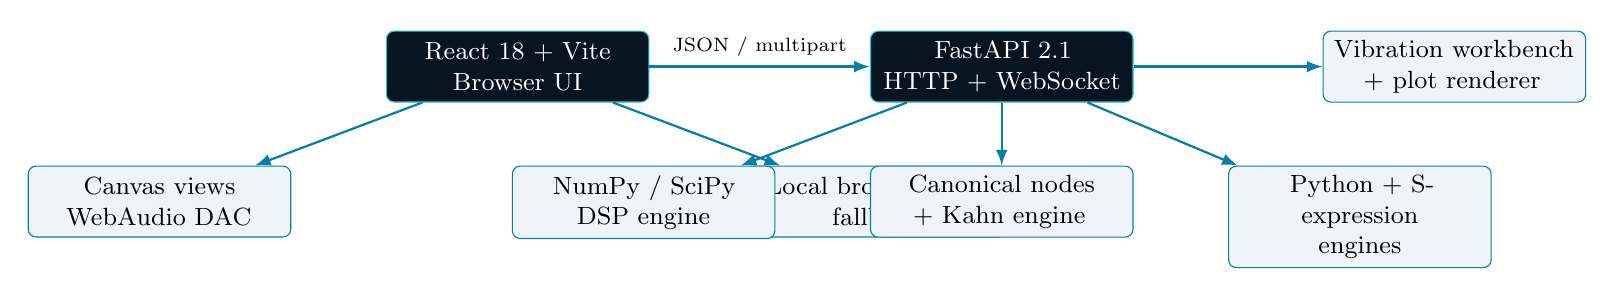
\begin{tikzpicture}[
  node distance=8mm and 12mm,
  box/.style={draw=RCBlue,fill=RCLight,rounded corners=1mm,align=center,minimum height=9mm,text width=31mm,font=\small},
  core/.style={box,draw=RCCyan,fill=RCNavy,text=white},
  arr/.style={-{Latex[length=2mm]},thick,draw=RCBlue}
]
\node[core] (ui) {React 18 + Vite\\Browser UI};
\node[box,below left=of ui] (canvas) {Canvas views\\WebAudio DAC};
\node[box,below right=of ui] (local) {Local browser DSP\\fallback};
\node[core,right=28mm of ui] (api) {FastAPI 2.1\\HTTP + WebSocket};
\node[box,below left=of api] (dsp) {NumPy / SciPy\\DSP engine};
\node[box,below=of api] (graph) {Canonical nodes\\+ Kahn engine};
\node[box,below right=of api] (script) {Python + S-expression\\engines};
\node[box,right=24mm of api] (render) {Vibration workbench\\+ plot renderer};
\draw[arr] (ui) -- node[above,font=\scriptsize]{JSON / multipart} (api);
\draw[arr] (ui) -- (canvas);
\draw[arr] (ui) -- (local);
\draw[arr] (api) -- (dsp);
\draw[arr] (api) -- (graph);
\draw[arr] (api) -- (script);
\draw[arr] (api) -- (render);
\end{tikzpicture}
}
\end{center}

The frontend orchestrates state, renders controls and instruments, submits work to the API, and can calculate a limited local fallback when the API is unavailable. The backend validates requests with Pydantic models, runs NumPy/SciPy processing, produces telemetry and spectrogram arrays, executes graph and scripting workflows, and returns structured results. Firebase Hosting serves the published web application; backend hosting is a separate deployment concern.

\subsection{Main source modules}

\begin{tabularx}{\textwidth}{L{4.1cm}Y}
\toprule
Module & Responsibility\\
\midrule
\code{frontend/src/App.jsx} & Application state, presets, upload/export actions, trust-mode switching, and workspace navigation.\\
\code{frontend/src/components/} & Oscilloscope, spectrum, waterfall, metrics, audio, controls, graph studio, Python/Lisp editors, and \code{VibrationWorkbench.jsx}.\\
\code{backend/app/main.py} & FastAPI application, request routes, upload parsing, exports, and streaming.\\
\code{backend/app/schemas.py} & Enumerations, validation constraints, request structures, and response models.\\
\code{backend/app/dsp_engine.py} & Generation, modulation, math stages, filtering, FFT, metrics, spectrograms, and plot rendering.\\
\code{backend/app/graph/} & Canonical port types, registry, graph validation, Kahn topological scheduling, deterministic execution, and telemetry.\\
\code{backend/app/nodes/} & Canonical DSP and vibration node specifications, aliases, factories, and runtime implementations.\\
\code{backend/app/python_engine.py} & Restricted Python namespace, output capture, plot capture, and result extraction.\\
\code{backend/app/lisp_engine.py} & S-expression parsing and the supported DSP macro dispatcher.\\
\bottomrule
\end{tabularx}

\subsection{Processing pipeline}

The standard \code{/api/process} route applies stages in a fixed order:

\begin{center}
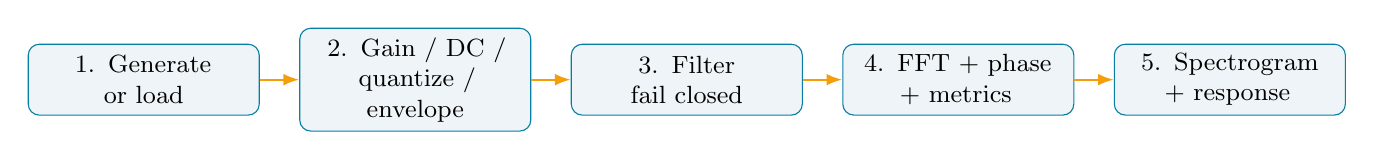
\begin{tikzpicture}[node distance=5mm,
  p/.style={draw=RCBlue,fill=RCLight,rounded corners,minimum height=9mm,text width=27mm,align=center,font=\small},
  a/.style={-{Latex[length=2mm]},thick,draw=RCOrange}]
\node[p] (g) {1. Generate\\or load};
\node[p,right=of g] (m) {2. Gain / DC /\\quantize / envelope};
\node[p,right=of m] (f) {3. Filter\\fail closed};
\node[p,right=of f] (x) {4. FFT + phase\\+ metrics};
\node[p,right=of x] (s) {5. Spectrogram\\+ response};
\draw[a] (g)--(m); \draw[a] (m)--(f); \draw[a] (f)--(x); \draw[a] (x)--(s);
\end{tikzpicture}
\end{center}

This order matters. For example, quantization noise is introduced before filtering, metrics describe the filtered signal, and the optional Hilbert envelope is derived at the math stage rather than after the filter.

\section{Getting started}

\subsection{Fastest browser workflow}

\begin{enumerate}
  \item Open the live application.
  \item Select a preset such as \emph{Sine 440 Hz}, \emph{AM Modulation}, \emph{Filtered Noise}, or \emph{ECG Telemetry}.
  \item Confirm the data-trust badge. Prefer \status{RCGreen}{API VERIFIED} for backend-calculated metrics.
  \item Adjust generator, math, filter, and FFT controls in the right-side panel.
  \item Inspect the waveform and spectrum. Open the waterfall view for time-varying spectral content.
  \item Use CSV export for numeric analysis or WAV export for audio playback and downstream tools.
\end{enumerate}

\subsection{Recommended first experiment}

Load the 440 Hz sine preset, keep the sample rate at 44.1 kHz, enable an eighth-order low-pass filter with a cutoff above 440 Hz, and compare the time and frequency plots. Then add noise and lower the cutoff. Observe how RMS, spectral floor, SNR, and SFDR change. Because FFT estimates depend on window, record length, and coherent sampling, treat small changes as configuration-dependent rather than absolute instrument specifications.

\subsection{Built-in presets}

\begin{tabularx}{\textwidth}{L{2.9cm}L{3.4cm}Y}
\toprule
Preset & Main configuration & Learning objective\\
\midrule
Sine 440 Hz & 440 Hz sine, 44.1 kHz, Hann, 1024 FFT & Baseline waveform and single-tone spectrum.\\
AM Modulation & 1 kHz carrier, 50 Hz modulation, index 0.8, envelope enabled & Sidebands and envelope extraction.\\
Filtered Noise & Gaussian noise, 800 Hz Butterworth low-pass & Broadband energy and filter response.\\
ECG Telemetry & 1.2 Hz synthetic ECG, DC removal, 40 Hz FIR low-pass & Slow biomedical-like waveform visualization; simulation only.\\
\bottomrule
\end{tabularx}

\section{User interface guide}

The interface uses a deliberately retro desktop-instrument visual language. The title bar identifies version 2.1; top-level tabs switch among the analysis workspaces; the toolbar provides file, export, and preset actions; and the control panel edits the active synthesis and processing configuration.

\subsection{Toolbar and common actions}

\begin{description}
  \item[Open File] Uploads \code{.wav}, \code{.csv}, \code{.txt}, or \code{.json}. Upload processing requires the backend.
  \item[Export CSV] Downloads columns for time, raw amplitude, and filtered amplitude from the current result.
  \item[Export WAV] Requests backend-generated normalized 16-bit PCM audio. If unavailable, the frontend can build a browser WAV from the displayed filtered signal.
  \item[Presets] Replaces the current generator, math, filter, and FFT configuration with a known example.
  \item[Audio engine] Uses WebAudio for local audible synthesis. Reduce volume before testing high-amplitude or noisy signals.
\end{description}

\subsection{Oscilloscope + Spectrum}

The dual view is the default measurement workspace. The oscilloscope plots raw, filtered, and optional envelope traces against time. The spectrum analyzer plots FFT magnitude against frequency and is accompanied by measurement telemetry. Use it to compare time-domain distortion with frequency-domain content.

Useful checks include:
\begin{itemize}
  \item verify that displayed frequency is below the Nyquist limit $f_s/2$;
  \item select a duration long enough to show low-frequency cycles;
  \item increase FFT size for finer bin spacing, while remembering that zero-padding does not add information;
  \item choose a flat-top window for amplitude-oriented work and Hann/Hamming for general leakage control;
  \item inspect the trust badge before recording metrics.
\end{itemize}

\subsection{Signal Flow Studio}

The 2.1 graph workspace composes processing as connected canonical nodes. Projects can be exported and imported as versioned JSON with the \code{.rei-signal} extension. The canvas supports node dragging and SVG cable wiring; Canvas-based scope and spectrum sinks can display pipeline results. The backend resolves canonical types and legacy aliases, applies compatibility checks to every connection, rejects cycles, and executes valid graphs deterministically with Kahn's topological scheduler.

The versioned catalog exposed by \code{GET /api/nodes} contains more than 35 nodes. Representative families include:

\begin{tabularx}{\textwidth}{L{2.7cm}L{5.2cm}Y}
\toprule
Category & Canonical examples & Purpose\\
\midrule
Generators & \code{generator.signal}, \code{generator.gaussian\_noise} & Synthesize standard waveforms and deterministic seeded Gaussian noise.\\
Arithmetic & \code{arithmetic.add}, \code{subtract}, \code{multiply}, \code{divide} & Combine real-valued signals sample by sample; division clamps zero denominators.\\
Filters & \code{filter.lowpass}, \code{highpass}, \code{biquad\_iir}, \code{median} & Apply IIR/FIR, pole-checked SOS, and impulse-noise filtering.\\
Transforms & \code{transform.fft}, \code{inverse\_real\_fft}, \code{dct}, \code{haar}, \code{hilbert} & Perform Fourier, cosine, Haar wavelet, and analytic-signal operations.\\
Converters & \code{converter.real\_to\_complex}, \code{complex\_to\_real} & Convert between real and complex signal representations.\\
Analysis & \code{analysis.noise\_stats}, \code{pattern\_detector}, \code{min\_max} & Compute telemetry, normalized correlation events, and amplitude extrema.\\
Vibration & \code{vibration.sensor\_calibration}, \code{bearing\_frequencies}, \code{envelope\_analysis}, \code{balance.single\_plane}, \code{fault\_classifier} & Calibrate sensors, derive machinery indicators, balance rotors, and classify fault evidence.\\
Generic & \code{generic.real\_value\_filter} & Evaluate a restricted mathematical expression through an AST allowlist without \code{exec} or \code{eval}.\\
\bottomrule
\end{tabularx}

Real-valued ports use \code{Signal<Real64>} and \code{Scalar<Real64>}; complex streams use \code{Signal<Complex128>}. Additional contracts include \code{SpectrumFrame}, \code{PatternEvent}, and structured frames. A connection is accepted only when its source and destination signatures are compatible. Legacy names such as \code{SLFourier}, \code{SLRMSMeter}, and \code{SLBearingFreqs} are aliases; new projects should persist canonical names.

\subsection{REI Vibration Analysis Workbench}

The new Vibration Analysis Workbench targets rotating-machinery condition monitoring and balancing. Its setup panel records machine name/type, shaft speed in RPM, sensor type and sensitivity, measurement axis, bearing element count, ball diameter, and pitch diameter. The visual area provides an acceleration waveform, FFT spectrum with 1X/2X and bearing-frequency markers, Hilbert envelope spectrum, a 1X--10X harmonic order bar view, and a rotor-balancing polar plot.

\begin{center}
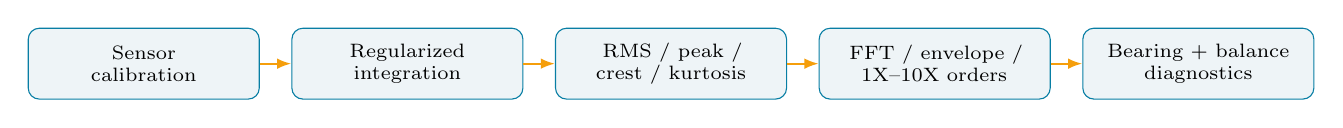
\begin{tikzpicture}[node distance=4mm,
  p/.style={draw=RCBlue,fill=RCLight,rounded corners,minimum height=9mm,text width=27mm,align=center,font=\scriptsize},
  a/.style={-{Latex[length=1.8mm]},thick,draw=RCOrange}]
\node[p] (c) {Sensor\\calibration};
\node[p,right=of c] (i) {Regularized\\integration};
\node[p,right=of i] (t) {RMS / peak /\\crest / kurtosis};
\node[p,right=of t] (e) {FFT / envelope /\\1X--10X orders};
\node[p,right=of e] (d) {Bearing + balance\\diagnostics};
\draw[a] (c)--(i); \draw[a] (i)--(t); \draw[a] (t)--(e); \draw[a] (e)--(d);
\end{tikzpicture}
\end{center}

For a shaft frequency $f_r=\mathrm{RPM}/60$, rolling-element count $N$, ball diameter $d$, pitch diameter $D$, and contact angle $\phi$, the bearing calculator derives cage and race frequencies. Two commonly used results are
\[
 \mathrm{BPFO}=\frac{N}{2}f_r\left(1-\frac{d}{D}\cos\phi\right),\qquad
 \mathrm{BPFI}=\frac{N}{2}f_r\left(1+\frac{d}{D}\cos\phi\right).
\]
The workbench also reports BSF and FTF, and marks these frequencies against the spectrum. Envelope demodulation is intended to reveal repetitive high-frequency impacts associated with rolling-element bearing faults.

Single-plane balancing uses the initial vibration vector, a known trial-weight vector, and the measured trial response to estimate an influence coefficient and a correction mass/angle. The rule-based classifier evaluates evidence for unbalance, angular/parallel misalignment, looseness, and bearing defects. The export action produces a JSON diagnostic report containing machine/sensor metadata, bearing frequencies, overall metrics, balance results, timestamp, and engine version.

\begin{warningbox}[title={Vibration data boundary}]
The current browser workbench synthesizes illustrative telemetry locally for its interactive displays; its random impact/noise samples and fixed demonstration harmonic bars are not acquired sensor measurements. Use backend canonical vibration nodes with validated input data for numerical workflows, retain calibration/provenance, and do not treat the browser demonstration or rule-based labels as a certified machinery diagnosis.
\end{warningbox}

\subsection{Python Lab}

Python Lab accepts signal-processing scripts, captures console output, extracts expected arrays, and converts a Matplotlib figure to a base64 PNG. The provided namespace includes \code{np}/\code{numpy}, SciPy signal functions as \code{signal} or \code{scipy\_signal}, \code{plt}, \code{matplotlib}, and standard variables such as \code{sample\_rate}.

A script can return plot and signal data by assigning \code{t}, \code{raw\_signal}, and \code{filtered\_signal}. Example:

\begin{lstlisting}[language=Python]
sample_rate = 44100
t = np.linspace(0, 0.1, int(sample_rate * 0.1), endpoint=False)
raw_signal = np.sin(2 * np.pi * 1000 * t)
b, a = signal.butter(4, 1800 / (sample_rate / 2), btype='low')
filtered_signal = signal.filtfilt(b, a, raw_signal)

plt.plot(t[:600], raw_signal[:600], label='raw')
plt.plot(t[:600], filtered_signal[:600], label='filtered')
plt.legend()
plt.title('1 kHz tone')
print('samples:', len(raw_signal))
\end{lstlisting}

\begin{warningbox}[title={Security boundary}]
The repository implements an application-level restricted namespace, blocked imports/keywords, and output caps. It executes Python with \code{exec} inside the API process; it is not a complete operating-system sandbox. Do not expose this endpoint to untrusted public users without separate process/container isolation, strict CPU and memory limits, timeouts, authentication, rate limiting, audit logs, and security review.
\end{warningbox}

\subsection{2D Waterfall}

The waterfall renders frequency content over time from the returned spectrogram matrix. It is especially useful for chirps, modulation, transient events, changing noise, and filter settling. Frequency occupies one axis, time the other, and color encodes magnitude. Confirm the axis limits and color scale before comparing two runs.

\subsection{S-Expression DSL Kernel}

The DSL parses a compact list syntax into an abstract syntax tree and applies recognized vector operations. Supported macros in the repository include:

\begin{itemize}
  \item \code{(biquad-filter-simd signal b0 b1 b2 a1 a2)}
  \item \code{(lisp-quantize-buffer signal bits)}
  \item \code{(lisp-convolve-simd signal-a signal-b)}
  \item \code{(apply-kaiser-window signal beta)}
\end{itemize}

Despite the naming, this is a purpose-built S-expression interpreter, not a general Common Lisp runtime. Only implemented macros and argument forms should be expected to work.

\section{Signal generation and processing}

\subsection{Waveform generator}

\begin{longtable}{L{3.2cm}L{3cm}L{8.2cm}}
\toprule
Waveform & API value & Description\\
\midrule
\endhead
Sine & \code{sine} & Single sinusoidal carrier.\\
Square & \code{square} & Symmetric two-level waveform rich in odd harmonics.\\
Triangle & \code{triangle} & Symmetric ramp waveform with decreasing odd harmonics.\\
Sawtooth & \code{sawtooth} & Linear ramp with integer harmonic content.\\
Gaussian noise & \code{noise} & Random normal samples. Runs are not deterministic unless external seeding is added.\\
Pink noise & \code{pink\_noise} & Frequency-shaped random noise approximating decreasing power with frequency.\\
Chirp & \code{chirp} & Linear sweep from \code{frequency} to \code{frequency2}.\\
ECG & \code{ecg} & Synthetic pulse morphology assembled from Gaussian components; educational simulation only.\\
Multitone & \code{multitone} & Fundamental plus secondary and fifth-frequency components at fixed relative amplitudes.\\
Pulse & \code{pulse} & Square-wave pulse train with approximately 10\% duty cycle.\\
\bottomrule
\end{longtable}

Generator constraints include frequency 0.1--20,000 Hz, amplitude 0--100, phase $-360^\circ$ to $360^\circ$, offset $-50$ to 50, sample rate 100--192,000 samples/s, duration 1 ms--10 s, and noise level 0--10. The practical frequency limit must also respect Nyquist and the desired transition band.

\subsection{Modulation}

The generator supports none, AM, FM, and PM modes. For a carrier $c(t)$ and sinusoidal modulator $m(t)$, the implementation broadly follows:

\begin{align*}
 y_{\mathrm{AM}}(t) &= A[1+I m(t)]c(t),\\
 y_{\mathrm{FM}}(t) &= A\sin(2\pi f_c t + I m(t)+\phi),\\
 y_{\mathrm{PM}}(t) &= A\sin(2\pi f_c t + I\cos(2\pi f_m t)+\phi),
\end{align*}

where $I$ is the configured modulation index. The FM implementation is a phase-argument modulation model; users needing standards-specific frequency deviation should validate the interpretation against their requirements.

\subsection{Math and quantization stage}

The math stage applies gain in decibels, optional mean subtraction, optional finite-level quantization, and optional Hilbert envelope extraction. Gain uses $10^{G/20}$. Quantization normalizes by peak absolute amplitude, maps samples into $2^b$ levels, then maps them back to the original peak range. This models amplitude quantization but not every behavior of a physical ADC.

\subsection{Filters}

Available response types are low-pass, high-pass, band-pass, and band-stop. Available designs are Butterworth, Chebyshev I, Chebyshev II, elliptic, Bessel, FIR window, and median. IIR and FIR branches use forward-backward filtering, giving zero-phase offline behavior rather than a causal real-time implementation.

\begin{tabularx}{\textwidth}{L{3cm}Y}
\toprule
Design & Typical use\\
\midrule
Butterworth & Smooth passband and general-purpose filtering.\\
Chebyshev I & Sharper transition with passband ripple.\\
Chebyshev II & Stopband ripple with a flatter passband.\\
Elliptic & Very sharp transition with ripple in both bands.\\
Bessel & Smooth time-domain behavior; validate digital normalization for the use case.\\
FIR window & Finite impulse response design; useful where FIR behavior is desired.\\
Median & Nonlinear suppression of impulsive outliers.\\
\bottomrule
\end{tabularx}

The engine clamps cutoffs below Nyquist, limits filter order to 1--10, checks designed IIR poles, and raises an error rather than silently returning raw input if filtering fails. This is the product's \emph{fail-closed} DSP policy.

\subsection{FFT configuration}

FFT length must be a positive power of two. Supported windows are rectangular, Hamming, Hanning/Hann, Blackman, Kaiser, and flat-top. The one-sided magnitude is corrected by the window sum, the DC term is halved, and logarithmic mode returns $20\log_{10}$ magnitude with a small floor to avoid $\log(0)$.

Nominal FFT bin spacing is
\[
\Delta f = \frac{f_s}{N_{\mathrm{FFT}}}.
\]
Actual resolvability also depends on observation duration, window main-lobe width, stationarity, and signal-to-noise ratio.

\section{Measurement telemetry}

\begin{tabularx}{\textwidth}{L{2.8cm}L{3.4cm}Y}
\toprule
Metric & Meaning & Implementation note\\
\midrule
RMS & Root-mean-square amplitude & Calculated directly from time samples.\\
Peak-to-peak & Maximum minus minimum & Sensitive to outliers and record length.\\
DC mean & Arithmetic mean & Indicates offset in the analyzed record.\\
Fundamental & Strongest non-DC FFT bin & Bin-centered estimate, not an interpolated estimator.\\
THD & Harmonic distortion ratio & Combines bins nearest harmonics 2 through 5 relative to the fundamental.\\
SNR & Signal-to-noise ratio & Uses spectral power after subtracting estimated fundamental and harmonics.\\
SINAD & Signal to noise and distortion & Fundamental power divided by combined noise and harmonic power.\\
SFDR & Spurious-free dynamic range & Fundamental amplitude relative to the largest remaining spectral bin.\\
ENOB & Effective number of bits & Computed as $(\mathrm{SINAD}-1.76)/6.02$, clamped at zero.\\
\bottomrule
\end{longtable}

These metrics are useful for comparative experiments, but their accuracy depends on coherent acquisition, correct scaling, adequate FFT length, window selection, anti-aliasing, and exclusion rules. The implementation is a compact estimator rather than a substitute for a standards-specific ADC or audio measurement procedure.

\section{Data trust and provenance}

SignalLab deliberately identifies where results were computed. This prevents a locally generated fallback from being mistaken for a backend-verified calculation.

\begin{trustbox}[title={API VERIFIED},fonttitle=\bfseries,coltitle=white]{RCGreen}
The FastAPI/SciPy backend completed the request. Full metrics and server processing are available. This label confirms computation origin, not calibration of the source hardware or compliance with a measurement standard.
\end{trustbox}

\begin{trustbox}[title={LOCAL BROWSER DSP},fonttitle=\bfseries,coltitle=white]{RCBlue}
The API was unavailable and the browser generated a simplified local result. The frontend fallback provides time data, a local spectrum, RMS, peak-to-peak, and DC; advanced telemetry fields may be unavailable. Record this mode in any exported research notes.
\end{trustbox}

\begin{trustbox}[title={DEMO MODE},fonttitle=\bfseries,coltitle=RCNavy]{RCOrange}
The display contains simulated demonstration data and must show a warning equivalent to: \emph{Simulated demo data---not for instrument measurement}. Do not cite these values as observations from physical equipment.
\end{trustbox}

For reproducible work, save the project and configuration, input file, trust mode, software version or commit, browser and backend environment, timestamp, and exported numeric data. For random noise, also save the actual output or add a controlled random seed in a custom workflow.

\section{Files, projects, and exports}

\subsection{Input files}

\begin{tabularx}{\textwidth}{L{2.2cm}Y}
\toprule
Format & Parsing behavior\\
\midrule
WAV & Reads 8-, 16-, or 32-bit samples; multi-channel audio is averaged to mono. Other sample widths follow a float fallback. Sample rate is taken from the WAV header.\\
JSON & Accepts a top-level numeric list or an object with \code{signal} or \code{data}; optional \code{sample\_rate}, default 44,100.\\
CSV/TXT & Reads lines separated by newline, accepts comma or tab-like separation, and uses the final numeric field on each usable line. Simple alphabetic headers are skipped.\\
\bottomrule
\end{tabularx}

Uploaded signals are truncated to 16,384 samples in the current backend. Empty or unsupported input returns a client error. Large, multi-column, irregular, compressed, or metadata-heavy datasets should be normalized before upload.

\subsection{The .rei-signal project format}

A graph project is versioned JSON containing a project ID, a sample clock, nodes, connections, and engine environment information.

\begin{lstlisting}[language={},caption={Minimal illustrative project}]
{
  "formatVersion": "2.1",
  "projectId": "example-project",
  "sampleClock": {"rateHz": 44100, "timebase": "monotonic"},
  "graph": {
    "nodes": [
      {"id": "src", "type": "generator.signal", "name": "Tone",
       "params": {"waveform": "sine", "frequency": 1000}},
      {"id": "fft", "type": "transform.fft", "name": "Spectrum",
       "params": {"n_fft": 2048}}
    ],
    "connections": [
      {"from_node": "src", "from_port": "signal_out",
       "to_node": "fft", "to_port": "signal_in"}
    ]
  },
  "environment": {"dspEngineVersion": "2.1.0"}
}
\end{lstlisting}

The 2.1 engine uses double-precision canonical signal and scalar types, plus complex signals, spectrum frames, pattern events, and structured frames. A spectrum output cannot be connected to a real-signal input. Validation covers node existence, unique IDs, port existence and direction, type compatibility, required inputs, duplicate connections, and cycles. Kahn's algorithm computes execution order; if not all nodes can be ordered, execution is rejected with HTTP 422.

\subsection{Exports}

CSV is the best choice for notebooks, spreadsheets, audit trails, and external plotting. WAV export creates mono, 16-bit PCM; the backend normalizes to full scale before conversion, so absolute amplitude is not preserved. Browser fallback WAV clamps displayed samples into $[-1,1]$. Always preserve CSV or configuration data if numeric amplitude matters.

\section{REST and WebSocket API}

The API uses JSON except for multipart upload and binary plot/WAV responses. A default FastAPI deployment also provides generated OpenAPI documentation at \code{/docs} and \code{/redoc}, unless disabled by the operator.

\begin{longtable}{L{1.5cm}L{4.3cm}L{9.6cm}}
\toprule
Method & Endpoint & Purpose\\
\midrule
\endhead
GET & \code{/} & Health/status response and feature manifest.\\
GET & \code{/api/nodes} & Return the versioned canonical node catalog, ports, parameters, documentation, and legacy aliases.\\
POST & \code{/api/process} & Full synthetic generation, math, filter, FFT, metrics, and spectrogram pipeline.\\
POST & \code{/api/upload/signal} & Multipart upload and processing for WAV, CSV, TXT, and JSON.\\
POST & \code{/api/graph/execute} & Validate and execute a typed \code{.rei-signal} project.\\
POST & \code{/api/python/execute} & Run an experimental restricted Python DSP script.\\
POST & \code{/api/lisp/process} & Apply supported S-expression DSP macros to a generated signal.\\
POST & \code{/api/render/plot} & Return a Matplotlib PNG for an oscilloscope or spectrum request.\\
GET & \code{/api/render/plot} & Render a PNG from query parameters.\\
POST & \code{/api/export/wav} & Return normalized mono 16-bit PCM WAV.\\
WS & \code{/ws/stream} & Stream 512 time samples and 256 spectral bins at a nominal loop delay of about 33 ms.\\
\bottomrule
\end{longtable}

\subsection{Numerical golden verification}

Version 2.1 adds reference-vector tests for the graph runtime and canonical numerical nodes. The published suite checks representative arithmetic and window operations at float64 tolerances near $10^{-12}$, FFT/inverse reconstruction RMS error near $10^{-9}$, and DCT Type II and Haar transform results near $10^{-12}$. It also exercises port validation, cycle detection, seeded noise reproducibility, expression-filter safety, and vibration formulas. These are software regression thresholds, not calibration or uncertainty specifications for external hardware.

\subsection{Process request example}

\begin{lstlisting}[language=bash]
curl -X POST "http://localhost:8000/api/process" \
  -H "Content-Type: application/json" \
  -d '{
    "generator": {
      "waveform": "multitone", "frequency": 1000,
      "frequency2": 1700, "amplitude": 1,
      "sample_rate": 44100, "duration": 0.2
    },
    "math": {"dc_remove": true, "gain_db": 0},
    "filter": {
      "enabled": true, "filter_type": "lowpass",
      "filter_design": "butterworth", "cutoff": 5000, "order": 4
    },
    "fft": {"n_fft": 4096, "window": "hanning", "log_scale": true}
  }'
\end{lstlisting}

\subsection{Response shape}

The standard response contains time, raw and filtered samples, optional envelope, FFT frequency/magnitude/phase arrays, a metrics object, and optional spectrogram frequency/time/matrix arrays. Arrays can be large; clients should avoid unnecessary UI rerenders and should enforce payload limits in production.

\subsection{Errors}

Pydantic validation errors normally produce HTTP 422. Graph validation errors also use 422. Unsupported or empty uploads produce 400. Processing, render, and runtime failures are generally returned as HTTP 500 with a descriptive detail field. Production gateways should avoid exposing internal exception detail if it might reveal sensitive implementation information.

\section{Local development}

\subsection{Prerequisites}

Use Python 3.11 or newer, Node.js with npm, and a modern browser. The repository's Python requirements and npm lockfile should be treated as the dependency authority.

\subsection{Backend}

\begin{lstlisting}[language=bash]
git clone https://github.com/rootcastleco/rei-signallab.git
cd rei-signallab
pip install -r backend/requirements.txt
PYTHONPATH=backend pytest backend/tests
PYTHONPATH=backend uvicorn app.main:app --port 8000 --reload
\end{lstlisting}

\subsection{Frontend}

In another terminal:

\begin{lstlisting}[language=bash]
cd rei-signallab/frontend
npm install
npm run dev
\end{lstlisting}

Open the Vite URL shown in the terminal, commonly \code{http://localhost:3000} in the repository documentation. Ensure the frontend API configuration points to the backend and that CORS policy matches the actual frontend origin.

\subsection{Testing checklist}

\begin{itemize}
  \item Run backend unit tests and frontend build checks.
  \item Exercise every waveform, filter design, and FFT window at boundary values.
  \item Verify a known pure tone against expected RMS, frequency bin, and magnitude.
  \item Test cycle and port-type rejection in the graph engine.
  \item Upload mono and stereo WAV plus representative CSV, TXT, and JSON.
  \item Confirm API-offline browser fallback and its trust label.
  \item Test WAV RIFF header, CSV row count, and project import/export round-trip.
  \item Apply abuse tests to scripting endpoints before any network exposure.
\end{itemize}

\section{Deployment and operations}

\subsection{Production topology}

A practical deployment separates static frontend hosting from the Python API. Terminate TLS at a managed proxy, restrict CORS to the published origins, place authentication and rate limits before expensive routes, and run scripting features in an isolated worker tier. WebSocket support must be enabled end to end.

\subsection{Minimum hardening actions}

\begin{enumerate}
  \item Replace wildcard CORS with explicit origins; review the combination of wildcard origin and credentials.
  \item Authenticate write/compute routes and set per-user quotas.
  \item Enforce request-body, upload, array-length, execution-time, and response-size limits at both proxy and application layers.
  \item Move Python execution into disposable, non-root, network-disabled containers or microVMs with read-only filesystems and strict CPU/memory/process limits.
  \item Disable Python Lab entirely where secure isolation is unavailable.
  \item Sanitize error responses and retain structured server logs with request IDs.
  \item Pin dependencies, scan images, and rebuild regularly.
  \item Add health, latency, error-rate, memory, CPU, WebSocket, and queue-depth monitoring.
  \item Back up project artifacts if persistence is added; the current core is primarily stateless.
\end{enumerate}

\subsection{Capacity considerations}

FFT, filtering, spectrogram generation, Matplotlib rendering, and Python execution are CPU- and memory-sensitive. Large concurrency can block a simple synchronous worker pool. Use bounded worker concurrency, separate queues for plots/scripts, caching for identical safe requests, and conservative array limits. WebSocket clients generate repeated DSP work and should have connection, message, and idle limits.

\subsection{Observability}

Record route, status, latency, input sample count, FFT size, filter design/order, trust mode, worker identity, and a correlation ID. Never log uploaded signal contents or scripts by default if they may contain proprietary research data. Track graph validation failures separately from runtime failures; validation errors often indicate user configuration problems, whereas runtime spikes may indicate regressions or abuse.

\section{Troubleshooting}

\begin{longtable}{L{4cm}L{5.2cm}L{6.2cm}}
\toprule
Symptom & Likely cause & Action\\
\midrule
\endhead
Badge shows LOCAL BROWSER DSP & API unreachable, CORS failure, or server error & Check backend URL, browser network panel, TLS, CORS, and API health. Do not expect advanced verified metrics.\\
Upload fails & Unsupported format, empty numeric data, malformed WAV/JSON, or backend offline & Normalize input, test a small file, confirm extension and health endpoint.\\
Filter returns an error & Invalid band edges, insufficient record length for \code{filtfilt}, or unstable/failed design & Lower order, lengthen record, move cutoff away from Nyquist, and inspect server detail.\\
Unexpected spectral leakage & Non-coherent record or unsuitable window & Increase duration, choose Hann/Blackman, or align tone frequency to an FFT bin.\\
Wrong amplitude after WAV export & Backend WAV is peak-normalized & Use CSV for absolute amplitude or apply documented external scaling.\\
Graph HTTP 422 & Cycle, missing node, or incompatible port types & Inspect connections; keep graph acyclic and connect matching types.\\
Python script rejected & Blocked keyword/import or missing expected variables & Use the provided numerical namespace and assign output arrays explicitly.\\
Python request hangs or consumes resources & In-process execution lacks strong isolation/time enforcement & Stop the worker, disable the route, and deploy an isolated, quota-controlled executor.\\
Waterfall looks duplicated or coarse & Browser fallback or short/simple spectrogram data & Confirm API VERIFIED mode, increase duration, and use a time-varying signal.\\
Aliasing appears & Signal content is at or above Nyquist & Increase sample rate or reduce input frequency and add appropriate anti-alias filtering.\\
\bottomrule
\end{longtable}

\section{Research and measurement practice}

For defensible experiments, define the question before adjusting controls. Keep a fixed baseline, vary one parameter at a time, and export numeric results rather than relying only on screenshots. Record sampling rate, duration, FFT length/window, filter design/order/cutoffs, generator parameters, input provenance, software version, and trust mode.

When comparing spectra, use identical axes and windows. When comparing amplitudes, avoid normalized WAV as the primary record. When measuring THD or SNR, choose a sufficiently long coherent record, prevent clipping, and verify that harmonics fall below Nyquist. For real hardware data, document the sensor, ADC, analog conditioning, calibration date, reference source, and environmental conditions.

\begin{warningbox}[title={Safety and regulated use}]
Synthetic ECG is not a diagnostic signal. SignalLab is not presented as a medical device, safety controller, certified RF instrument, or calibration standard. Any regulated, safety-critical, clinical, or compliance use requires independent validation, risk management, qualified hardware, and the applicable approval process.
\end{warningbox}

\section{Extending the system}

\subsection{Adding a waveform}

Add the enum value and validation model, implement generation in \code{DSPEngine.generate\_signal}, expose controls in the frontend, provide a preset or test fixture, and test amplitude, phase, duration, Nyquist behavior, randomness, and serialization.

\subsection{Adding a graph node}

Define a canonical type name, explicit input/output \code{PortSpec} signatures, parameter schema, documentation, and any legacy aliases. Register the \code{NodeSpec}, implement its runtime/factory mapping, expose it through \code{/api/nodes}, update the UI palette and parameter editor, and add golden tests for missing inputs, invalid parameters, fan-in/fan-out, port mismatch, cycle behavior, determinism, and serialization.

\subsection{Adding a metric}

Specify the estimator and its assumptions first. Add the backend response field, implement and test with known reference vectors, update browser fallback only if an equivalent local estimator is appropriate, expose the metric with units and trust provenance, and document edge cases such as silence, DC, clipping, and multiple equal peaks.

\subsection{Compatibility discipline}

Treat \code{formatVersion}, API schemas, enum strings, port names/types, and result units as public contracts. Use additive changes where possible. For breaking project changes, provide migration and preserve the original file. Include engine version and, ideally, commit ID in exported provenance.

\section{Known limitations and roadmap considerations}

\begin{itemize}
  \item The public project describes instrument-grade intent, but software output is not equivalent to calibrated hardware measurement.
  \item The Python runner is not a strong security sandbox in its current in-process form.
  \item Canonical graph coverage has expanded substantially, but each node and alias should still be verified against the exact deployed backend revision before production use.
  \item The canonical Gaussian-noise graph node supports deterministic seeding; the older general processing request and browser vibration demonstration do not provide equivalent end-to-end reproducibility.
  \item The Vibration Workbench's interactive browser telemetry is synthesized demonstration data, and its rule-based classifier is not a standards-certified diagnostic system.
  \item Uploads are truncated to 16,384 samples and CSV parsing intentionally favors simple numeric files.
  \item Backend WAV export normalizes amplitude; it is not a bit-exact export of physical units.
  \item The WebSocket loop uses default configurations after short receive timeouts, so client protocol and desired continuity should be validated for production streaming.
  \item Current metric estimators are compact and bin-based rather than standards-specific measurement suites.
\end{itemize}

High-value future work includes isolated job execution, authentication and quotas, deterministic seeds across every signal path, fuller runtime parity for catalog aliases and UI controls, project schema migrations, calibration/uncertainty metadata, unit-aware signals, real sensor acquisition, streaming state continuity, batch processing, standards-specific vibration and spectral metric modes, and automated end-to-end reference-signal tests.

\section{Glossary}

\begin{longtable}{L{3cm}L{12.5cm}}
\toprule
Term & Definition\\
\midrule
\endhead
ADC & Analog-to-digital converter.\\
DAC & Digital-to-analog converter; WebAudio acts as the local playback path here.\\
DSP & Digital signal processing.\\
ENOB & Effective number of bits inferred from SINAD.\\
FFT & Fast Fourier transform, used to estimate frequency content.\\
FIR / IIR & Finite / infinite impulse response filter families.\\
Nyquist frequency & Half the sampling rate; sampled content above it aliases into lower frequencies.\\
RMS & Root-mean-square amplitude.\\
SFDR & Ratio between the fundamental and largest spurious spectral component.\\
SINAD & Ratio of signal to combined noise and distortion.\\
SNR & Signal-to-noise ratio.\\
Spectrogram & Magnitude as a function of both time and frequency.\\
THD & Total harmonic distortion.\\
Topological order & An ordering where every node runs after its dependencies; possible only for an acyclic graph.\\
Trust mode & UI provenance label identifying backend, browser, or demo computation origin.\\
Window & Weighting function applied before an FFT to manage leakage and amplitude tradeoffs.\\
\bottomrule
\end{longtable}

\section{Source and maintenance notes}

This document was prepared from the live application, the public \code{rootcastleco/rei-signallab} repository (README and source modules), and RootCastle's public website. Product facts should be revalidated when the repository version, deployed API, or project format changes.

\begin{tabularx}{\textwidth}{L{3.7cm}Y}
\toprule
Reference & URL\\
\midrule
Live application & \url{https://signallab-3305b.web.app/}\\
Repository and README & \url{https://github.com/rootcastleco/rei-signallab}\\
RootCastle & \url{https://rootcastle.com}\\
\bottomrule
\end{tabularx}

\vfill
\begin{center}
\textcolor{RCNavy}{\Large\bfseries ROOTCASTLE}\\[1mm]
\textcolor{RCBlue}{Engineering Beyond Boundaries}\\[2mm]
\small \product{} Product Wiki \textbullet\ Version 2.1 \textbullet\ August 2026
\end{center}

\end{document}
